\documentclass[a4paper, 11pt]{article}
\usepackage[top=3cm, bottom=3cm, left = 2cm, right = 2cm]{geometry}
\usepackage[brazilian]{babel}
\usepackage{setspace}
\usepackage{graphicx}
\usepackage{multicol}

\title{Relatório: Trabalho Final - MIPS Pipeline}
\author{Luize Cunha Duarte - GRR20221232\\
    Gabriel Lisboa Conegero - GRR20221255\\
    Pedro Folloni Pesserl - GRR20220072\\
    Rebeca Soares de Oliveira - GRR20221260\\
\textit{Departamento de Informática}\\
\textit{Universidade Federal do Paraná - UFPR}\\
Curitiba, Brasil\\
\texttt{lcd22@inf.ufpr.br, glc22@inf.ufpr.br,}\\
\texttt{pfp22@inf.ufpr.br, rso22@inf.ufpr.br}}
\date{}

\begin{document}
\maketitle

\begin{abstract}
\begin{singlespace}
Este relatório documenta o processo de implementação do processador MIPS Pipeline de 16
bits para FPGA (Field Programmable Gate Array) através da linguagem VHDL (VHSIC Hardware
Description Language). O projeto do processador possui uma memória de dados e uma
memória de instruções de 128 KiB cada, e um banco de registradores com quatro
registradores. 
\end{singlespace}
\end{abstract}

\section{As Instruções.}
As divisões dos bits para os endereços e funcionalidades das instruções foi pensada
visando evitar bits soltos e manter um espaço considerável para cada funcionalidade.
Por isso, as instruções seguem a base do MIPS, tendo sua divisão reorganizada para
16 bits.
\begin{itemize}
    \item Tipo R (opcode: 3 bits; rs: 2 bits; rt: 2 bits; rd: 2 bits; shamt: 4 bits;
        func: 3 bits).
        \begin{figure}[h]
        \centering
        
\includegraphics[width=.6\textwidth]{tipo-r.png}
        \caption{Formato das instruções do tipo R.}
        \end{figure}

    \item Tipo I. (opcode: 3 bits; rs: 2 bits; rt: 2 bits; imediato: 9 bits).
        \begin{figure}[h]
        \centering
        
\includegraphics[width=.6\textwidth]{tipo-i.png}
        \caption{Formato das instruções do tipo I.}
        \end{figure}
\end{itemize}
As instruções suportadas são:
\begin{multicols}{4}
\begin{itemize}
        \item ADD
        \item AND
        \item OR 
        \item NOR
        \columnbreak
        \item Set Less Than
        \item Shift Left Logical
        \item Shift Right Logical
        \item ADDI
        \columnbreak
        \item ANDI
        \item Display
        \item ORI
        \columnbreak
        \item Branch On Equal
        \item Load Word
        \item Store Word
\end{itemize}
\end{multicols}

\section{A arquitetura e sua implementação.}
Buscando uma arquitetura que suportasse todas as instruções decididas, sua organização
deu-se da maneira representada abaixo. Nesse sentido, cada componente foi implementado
utilizando a linguagem VHDL.

\begin{figure}[h!]
    \centering
    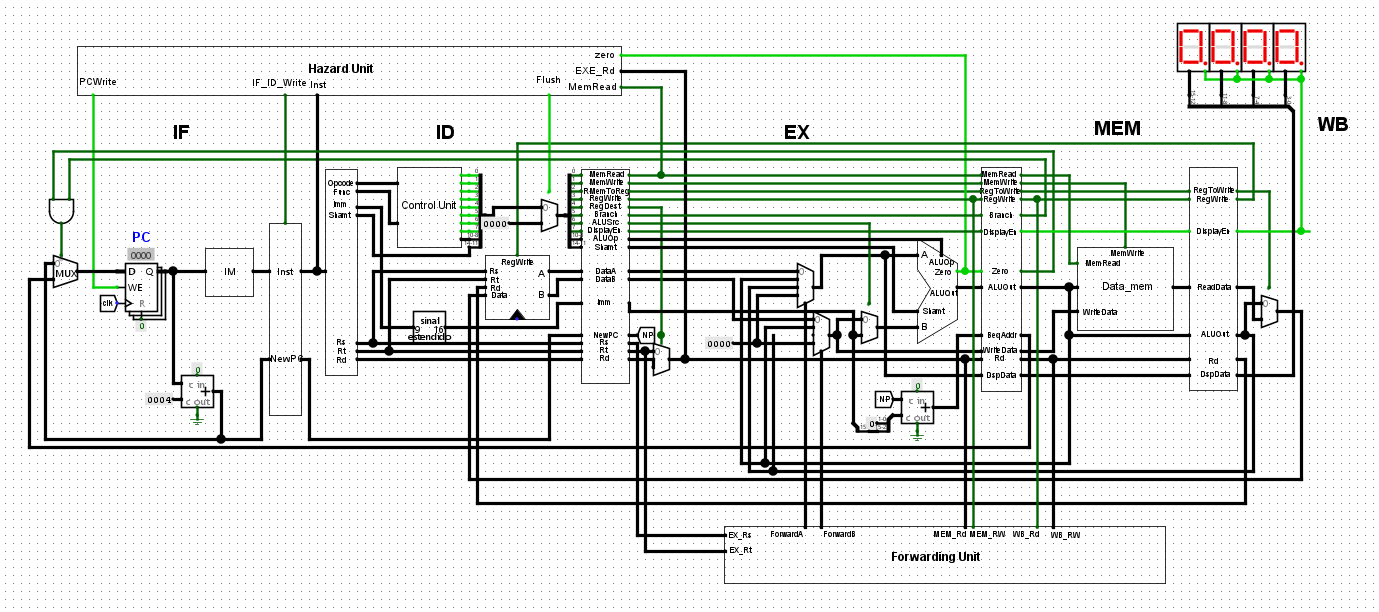
\includegraphics[width=.9\linewidth]{arquitetura.png}
    \caption{Bloco operacional do MIPS Pipeline.}
\end{figure}

\section{Os Componentes.}
\begin{enumerate}
    \item \textbf{Instruction Fetch}.

    Sendo a primeira parte da execução de uma instrução, é onde o ponteiro para a
    memória de instruções (Instruction Memory) é calculado e ela é lida, guardando tal instrução e sua localização no registrador intermediário IF\_ID. O PC pode ser atualizado para a próxima instrução, somando dois, ou para o endereço do Branch.

    \item \textbf{Instruction Decode}.

    Após lida, a instrução será decodificada, gerando seus sinais de controle através
    da Control Unit, a qual recebe os três primeiros bits e retorna os sinais necessários
    ligados. Além disso, os registradores usados para realizar a operação desejada são
    lidos no Register Bank, que possui quatro registradores de 16 bits de capacidade,
    sendo o primeiro sempre 0. Por fim, tem-se também nesse estágio a Hazarding Unit,
    a qual reconhece se a instrução sendo executada na proxima etapa irá desviar o fluxo
    de instruções, zerando as instruções que não serão mais executadas, um processo
    denominado “flush”.

    \item \textbf{Execute}.

    Tendo os dados necessários para realizar a operação, nessa etapa temos a ULA,
    controlada pela ALUControl, a qual verifica se é uma instrução do tipo R para
    realizar o “func” – últimos três bits da instrução – ou então uma soma,
    subtração, AND ou OR.

    Nessa parte, também a calculado o endereço do Branch on Equal,  bastando concatenar
    “00” ao fim do immediato extendido (bits 13 ao 0) e somar ao novo PC, passado pelos
    registradores intermediarios. Por fim, um componente importante para o desempenho do
    pipeline, a Forwarding Unit, é implementado na etapa. Esse componente é responsável
    por evitar stalls no processador ao receber dados de etapas seguintes, não sendo
    necessária a espera da escrita nos registradores – detalhada mais a frente – das
    instruções anteriores.

    \item \textbf{Memory}.

    O único componente presente é a memória de dados (Memory Data), o componente mais
    lento do Pipeline. Usada apenas nas funções de Load Word e Store Word, a memória
    possui 512 Bytes de armazenamento com 16 bits cada linha. Por fim, os dados carregados
    são passados para o registrador intermediário MEM\_WB.
    
    \item \textbf{Write-Back}.

    Sendo a última etapa do MIPS Pipeline, ela guarda no banco de registradores o
    dado de saída da ALU ou a palavra carregada da Memory Data. Por fim, o display também é acessado.
\end{enumerate}

\section{O Clock.}
    O Pipeline opera a uma frequência diferente do FPGA, tendo um clock mais lento que facilite a visualização de seu funcionamento. Para garantir isso, foi criado um componente para calcular o novo clock que será utilizado por todo o circuito.

\section{O Programa de Teste.}
    Foi escrito um programa simples como teste das funcionalidades do MIPS Pipeline. O 
    programa calcula os 10 primeiros números da sequência de Fibonacci, e cria sinais de
    saída para displays de sete segmentos, para cada dígito dos resultados.

\end{document}
